\chapter{Pendahuluan}
\authors{Alfa Yohannis, Rizki Wahyudi, Tommy Chitiawan, Mandalan}


	\gny{Tolong tambahkan keterangan gambar contoh : Gambar 7.1, 7.2, dst.. dan tambahkan italic text untuk setiap bahasa asing}

	\section{Definisi}
		\textit{Pipe and Filter Architecture} adalah sebuah pendekatan desain perangkat lunak yang menggambarkan bagaimana data dapat diproses melalui serangkaian \textit{filter} atau pemroses yang saling terkait dan saling bergantung dalam suatu \textit{pipeline}. Setiap \textit{filter} memiliki tugas spesifik untuk mengubah atau memanipulasi data yang melewatinya, dan data tersebut kemudian dikirim ke \textit{filter} berikutnya dalam \textit{pipeline} untuk diproses lebih lanjut.
	
	\textit{Pipe and Filter Architecture} terdiri dari beberapa elemen utama, yaitu:
	\begin{itemize}
		\item \textit{Pipes}: adalah saluran yang menghubungkan antara satu \textit{filter} dengan \textit{filter} lainnya. Pipe digunakan untuk mengalirkan data dari satu \textit{filter} ke \textit{filter} berikutnya.
		\item \textit{filter}: adalah blok bangunan logika yang bertanggung jawab untuk memproses dan mengubah data. \textit{Filter} dapat melakukan tugas sederhana seperti memisahkan atau menyaring data, atau tugas yang lebih kompleks seperti mengubah format data.
		\item \textit{Source dan Sink}: adalah elemen yang menghasilkan \textit{input} data dan menerima \textit{output} data dari \textit{pipeline}.
	\end{itemize}
	
	Keuntungan utama dari \textit{Pipe and Filter Architecture} adalah bahwa ia memungkinkan pengembang untuk membangun sistem yang sangat modular, dengan setiap \textit{filter} melakukan tugas yang jelas dan terbatas. Hal ini membuat perubahan pada pipeline lebih mudah dan aman, karena hanya memerlukan perubahan pada satu \textit{filter} tanpa mempengaruhi \textit{filter} lainnya. Selain itu, arsitektur ini juga dapat meningkatkan kinerja sistem, karena memungkinkan untuk memproses data secara paralel dalam beberapa \textit{filter}.
	
	Namun, kelemahan dari \textit{Pipe and Filter Architecture} adalah bahwa dapat menjadi sulit untuk menangani kasus penggunaan yang kompleks, karena setiap filter harus dirancang dengan sangat baik agar dapat berjalan dengan benar dalam pipeline. Selain itu, pengembang harus memperhatikan antarmuka antara filter yang berbeda agar dapat saling berinteraksi dengan benar.
	
	
	\section{\textit{Pipe and Filter Architecture Schema}}
		\begin{figure}[h] 
		\begin{center} 
			\renewcommand{\figurename}{Gambar} 
			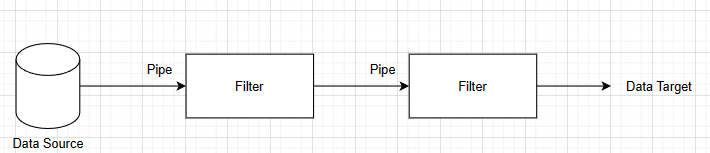
\includegraphics[scale=0.5]{Capture.png} 
			\caption{\textit{pipe and filter}} 
			\label{gambar} 
		\end{center} 
	\end{figure}
	
	\section{Kelebihan}
	
	\begin{itemize}
		\item Memastikan sambungan komponen, \textit{filter} yang longgar dan fleksibel.
		\item Kopling longgar memungkinkan \textit{filter} diubah tanpa modifikasi ke \textit{filter} lain.
		\item Konduktif untuk pemrosesan paralel.
		\item\textit{filter} dapat diperlakukan sebagai kotak hitam. Pengguna sistem tidak perlu mengetahui logika di balik kerja setiap \textit{filter}.
		\item Dapat digunakan kembali. Setiap \textit{filter} dapat dipanggil dan digunakan berulang kali.
	\end{itemize}
	
	
	\section{Kekurangan}
	
	\begin{itemize}
		\item Penambahan sejumlah besar \textit{filter independent} dapat mengurangi kinerja karena overhead komputasi yang berlebihan.
		\item Bukan pilihan yang baik untuk sistem interaktif.
		\item Sistem \textit{pipe and filter} mungkin tidak cocok untuk perhitungan jangka panjang.
		
	\section{penerapan dalam aplikasi}
		\begin{itemize}
			\item Sistem pengolahan data: \textit{Pipe and filter} dapat digunakan untuk mengambil data dari berbagai sumber dan memprosesnya melalui serangkaian \textit{filter} untuk menghasilkan \textit{output} yang diinginkan.
			
			\item Sistem pengolahan gambar: \textit{Pipe and filter} dapat digunakan untuk memproses gambar atau video yang diambil dari kamera dengan menggunakan berbagai filter untuk menghasilkan gambar yang lebih baik atau memberikan efek khusus.
			
			\item Sistem pencarian: \textit{Pipe and filter} dapat digunakan untuk memproses data pencarian yang diberikan oleh pengguna dan memfilter data untuk menghasilkan hasil pencarian yang relevan.
			
			\item Sistem pemrosesan audio: \textit{Pipe and filter} dapat digunakan untuk memproses audio dan melakukan pengolahan suara seperti pengurangan kebisingan, pengaturan volume, dan pemotongan audio.
			
			\item Sistem pemrosesan teks: \textit{Pipe and filter} dapat digunakan untuk memproses teks dan melakukan pengolahan bahasa alami seperti analisis sentimen dan pengenalan entitas.
		\end{itemize}
	\end{itemize}

